% Chapter 11: Linear Temporal Logic
% Sources: Course 89, L13-L17

\chapter{Linear Temporal Logic}
\label{ch:ltl}

In Part~I and the opening chapters of Part~II, we established the mathematical theory of automata over infinite words, specifically non-deterministic B\"uchi automata (NBA), and logical systems like $S1S$ (Monadic Second-Order Logic of One Successor). We proved B\"uchi's Theorem: $S1S$ and B\"uchi automata are expressively equivalent, defining the class of $\omega$-regular languages. 

However, compiling specifications written in $S1S$ is practically intractable due to its non-elementary decision complexity (characterized by a tower of exponentials of unbounded height). Furthermore, writing specifications in $S1S$ is highly error-prone. 

To bridge the gap between declarative convenience and algorithmic efficiency, we introduce \emph{Linear Temporal Logic (LTL)}, proposed by Amir Pnueli in 1977. LTL is a modal logic designed to specify properties over linear, infinite paths. It serves as the standard specification language in industrial model checking. In this chapter, we develop the syntax and semantics of LTL, analyze its expressive boundaries (star-free languages), prove the exponential succinctness of past-time operators, and detail the graph-theoretic tableau decision procedure for LTL satisfiability.

% =======================================================================
% =======================================================================
\section{The Logic of Linear Time}
\label{sec:ltl-motivation}

A temporal logic is characterized by how it represents the flow of time. In LTL, we assume a \emph{linear-time} model: at each moment, there is a single, unique future. This corresponds to evaluating formulas along a single execution path of a system.

Before formalizing the syntax and semantics of LTL, we establish its place in the broader context of software and hardware verification.

\subsection{Modal Logic Foundations}
Before we define the syntax of LTL, it is helpful to look at its roots. LTL is a specific flavor of \emph{modal logic}. Let's step up to the whiteboard and draw a Kripke structure: a graph of "multiple worlds." 
Imagine a 3-node graph with states $s_0, s_1, s_2$ connected by directed edges representing an "accessibility relation" (which worlds are reachable in one time-step from another). In standard modal logic, we evaluate formulas at a specific state. We have two key operators:
\begin{itemize}
    \item \textbf{Necessity ($\Box P$):} $P$ is true in \emph{all} immediately accessible neighboring worlds.
    \item \textbf{Possibility ($\Diamond P$):} $P$ is true in \emph{at least one} immediately accessible neighboring world.
\end{itemize}
This branching-world view is very expressive, but sometimes we want to study just a single execution trace of a system. What happens if we restrict our "multiple worlds" graph to be just an infinite linear chain of states ($s_0 \to s_1 \to s_2 \to \dots$)? On a linear chain, "all accessible worlds" and "some accessible world" collapse into exactly one world: the unique next state! This restriction gives birth to Linear Temporal Logic. The $\Box$ (always) and $\Diamond$ (eventually) operators are extended to evaluate properties over the entire infinite sequence rather than just the immediate neighbors.

\subsection{Verification vs. Validation}
In formal methods, we distinguish between two fundamental activities:
\begin{itemize}
    \item \textbf{Verification} (``Are we building the product right?''): The process of proving that a system meets its formal specification. It compares the system model against a set of mathematically defined properties.
    \item \textbf{Validation} (``Are we building the right product?''): The process of ensuring that the system meets the actual needs and expectations of the user. It checks the specifications themselves against the informal, real-world requirements.
\end{itemize}

\subsection{Historical Motivation: Classic Software and Hardware Bugs}
The necessity of formal verification is underscored by high-profile software and hardware failures where testing failed to uncover critical, edge-case bugs:
\begin{enumerate}
    \item \textbf{Therac-25 (1985--1987)}: A computerized radiation therapy machine that, due to software race conditions and a lack of hardware interlocks, administered massive radiation overdoses to patients, resulting in severe injuries and deaths.
    \item \textbf{AT\&T Network Outage (1990)}: A single buggy line of C code in a switch recovery routine caused a cascading crash, bringing down AT\&T's long-distance telephone network for 9 hours and disrupting 70 million calls.
    \item \textbf{Ariane 5 Flight 501 (1996)}: The rocket self-destructed 37 seconds after launch due to an unhandled integer overflow. A 64-bit floating-point variable representing horizontal velocity was cast into a 16-bit signed integer, causing the guidance software to fail.
\end{enumerate}

\subsection{Broader AI Applications of LTL}
While software verification is the primary driver for LTL, the logic has deep roots in Artificial Intelligence. Because LTL can concisely describe sequences of events and eventual goals, it is widely used in:
\begin{itemize}
    \item \textbf{Automated Planning}: Finding a sequence of robot actions that satisfies an LTL goal specification.
    \item \textbf{Automated Synthesis}: Compiling an LTL specification directly into a correct-by-construction reactive system.
    \item \textbf{Reinforcement Learning}: Using LTL formulas as reward functions to train agents, or as "shields" to prevent agents from taking unsafe actions during exploration.
\end{itemize}

\subsection{Dimensions and Classification of Temporal Logics}
Temporal logics can be classified along five main dimensions:
\begin{enumerate}
    \item \textbf{Qualitative Time vs. Real-Time}: 
          \emph{Qualitative} logics focus on the relative order of events (e.g., ``event $P$ happens before $Q$'' or ``$P$ eventually holds''). LTL is qualitative. \emph{Real-time} logics associate a numerical timestamp $t_i \in \mathbb{R}$ with each state $s_i$. To be physically meaningful, timestamps must satisfy \emph{monotonicity} ($t_i \le t_{i+1}$) and \emph{progress} (ruling out Zeno behaviors where infinitely many events occur in a finite interval of time, e.g., timestamps $4.3, 4.33, 4.333, \dots$ converging to $4.\overline{3}$ seconds). Formally, progress is enforced by the non-Zeno condition: $\lim_{i\to\infty} t_i = \infty$.
    \item \textbf{Discrete Time vs. Dense Time}:
          In \emph{discrete} time, the state sequence is isomorphic to $\mathbb{N}$: every point has a unique, immediate successor ($+1$), making the Next operator ($X$) well-defined. In \emph{dense} time (isomorphic to $\mathbb{R}$ or $\mathbb{Q}$), the concept of a successor is meaningless. LTL assumes discrete time.
    \item \textbf{Point-Based vs. Interval-Based}:
          \emph{Point-based} logics evaluate formulas at individual states. LTL is point-based. \emph{Interval-based} logics evaluate formulas over durations (e.g., ``property $P$ holds throughout interval $I$'').
    \item \textbf{Pure Future vs. Past and Future}:
          \emph{Pure future} logics only refer to states ahead of the current evaluation point. Logics with past operators can look backward in time.
    \item \textbf{Propositional vs. First-Order}:
          \emph{Propositional} logics evaluate formulas over sets of boolean variables. LTL is propositional.
\end{enumerate}

\medskip\noindent
\textbf{The $\omega$-Regular Connection.} 
By Kamp's Theorem (1968), LTL corresponds precisely to the \emph{first-order fragment of S1S} ($FO(S1S)$). This fragment defines exactly the \emph{star-free} $\omega$-regular languages (languages definable by $\omega$-regular expressions without using the Kleene star). 

\medskip\noindent
\textbf{Fairness preview.}
When LTL is used to describe executions of concurrent systems, it is common to talk about fair paths.  The two standard terms are \emph{justice} or weak fairness, for actions that stay enabled and should eventually occur, and \emph{compassion} or strong fairness, for actions that are enabled infinitely often and should also occur infinitely often.  Chapter~\ref{ch:ltl-mc-fairness} uses that terminology in the model-checking setting.

% =======================================================================
\section{Formal Syntax and Semantics of LTL}
\label{sec:ltl-formal}

Let $AP$ be a fixed, finite set of atomic propositions. The alphabet of our traces is $\Sigma = 2^{AP}$. 

\begin{definition}[LTL Syntax]
\label{def:ltl-syntax}
The formulas of Linear Temporal Logic (LTL) are defined inductively by the grammar:
\[
  \phi ::= p \mid \neg \phi \mid \phi_1 \land \phi_2 \mid X \phi \mid \phi_1 U \phi_2
\]
where $p \in AP$.
\end{definition}

Other boolean connectives are derived as standard shortcuts: $\top \equiv p \lor \neg p$, $\bot \equiv \neg \top$, $\phi_1 \lor \phi_2 \equiv \neg(\neg\phi_1 \land \neg\phi_2)$, and $\phi_1 \implies \phi_2 \equiv \neg\phi_1 \lor \phi_2$.

The temporal operators are:
\begin{itemize}
    \item $X \phi$ (``Next'' or ``Tomorrow''): $\phi$ must hold in the immediate successor state.
    \item $\phi_1 U \phi_2$ (``Until''): $\phi_2$ must eventually hold, and $\phi_1$ must hold continuously up to that point.
\end{itemize}

An LTL formula is interpreted over an infinite sequence of states, called a \emph{trace}. A trace $\sigma$ is an infinite word over $\Sigma$:
\[
  \sigma = s_0 s_1 s_2 \dots \in (2^{AP})^\omega
\]
where $s_i \subseteq AP$ is the set of propositions true at step $i$. We denote the suffix $s_i s_{i+1} s_{i+2} \dots$ as $\sigma[i..]$.

\begin{definition}[LTL Semantics]
\label{def:ltl-semantics}
The satisfaction relation $\sigma, i \models \phi$ (trace $\sigma$ satisfies $\phi$ at position $i \ge 0$) is defined inductively:
\begin{align*}
  \sigma, i &\models p &&\iff p \in s_i \quad (\text{for } p \in AP) \\
  \sigma, i &\models \neg \phi &&\iff \sigma, i \not\models \phi \\
  \sigma, i &\models \phi_1 \land \phi_2 &&\iff \sigma, i \models \phi_1 \text{ and } \sigma, i \models \phi_2 \\
  \sigma, i &\models X \phi &&\iff \sigma, i+1 \models \phi \\
  \sigma, i &\models \phi_1 U \phi_2 &&\iff \exists j \ge i \text{ such that } \sigma, j \models \phi_2 \text{ and } \forall k \in [i, j-1], \sigma, k \models \phi_1
\end{align*}
\end{definition}

\medskip\noindent
\textbf{Operational meaning of Semantics.} Let's decode this operationally. Evaluating $p$, $\neg\phi$, or $\phi_1 \land \phi_2$ at position $i$ just means looking at the state $s_i$ in isolation. The temporal magic happens with $X$ and $U$. The $X \phi$ operator simply shifts the evaluation pointer one step into the future to $i+1$. The $\phi_1 U \phi_2$ operator is a search loop: it looks for a future position $j$ where the goal $\phi_2$ is met, while simultaneously checking that the condition $\phi_1$ is unbroken for every step between $i$ and $j-1$.

\subsection{Derived Temporal Operators}
We define three crucial temporal operators as syntactic sugar:
\begin{itemize}
    \item \textbf{Eventually} ($F$): $F \phi \equiv \top U \phi$.
          \[
            \sigma, i \models F \phi \iff \exists j \ge i \text{ such that } \sigma, j \models \phi
          \]
    \item \textbf{Globally} ($G$): $G \phi \equiv \neg F \neg \phi$.
          \[
            \sigma, i \models G \phi \iff \forall j \ge i, \sigma, j \models \phi
          \]
    \item \textbf{Release} ($R$): The dual of Until. $\phi_1 R \phi_2 \equiv \neg(\neg\phi_1 U \neg\phi_2)$.
          \[
            \sigma, i \models \phi_1 R \phi_2 \iff \forall j \ge i, \left( \forall k \in [i, j], \sigma, k \not\models \phi_1 \right) \implies \sigma, j \models \phi_2
          \]
          Release requires that $\phi_2$ holds up to and including the point where $\phi_1$ becomes true; if $\phi_1$ never becomes true, $\phi_2$ must hold forever.
\end{itemize}

A trace $\sigma$ satisfies $\phi$, written $\sigma \models \phi$, if and only if $\sigma, 0 \models \phi$. The language of $\phi$ is $\mathcal{L}(\phi) = \{ \sigma \in (2^{AP})^\omega \mid \sigma \models \phi \}$. 
A formula $\phi$ is \emph{satisfiable} if $\mathcal{L}(\phi) \neq \emptyset$, and \emph{valid} (a tautology) if $\mathcal{L}(\phi) = (2^{AP})^\omega$.

% =======================================================================
\section{Equivalences and Temporal Expansions}
\label{sec:ltl-equivalences}

LTL formulas satisfy several algebraic dualities and expansion rules.

\subsection{Duality of Next and Eventually}
The operators $F$ and $X$ commute:
\[
  F X \phi \equiv X F \phi
\]
\begin{proof}
Let $\sigma \in \Sigma^\omega$ and $i \ge 0$.
\begin{align*}
  \sigma, i \models F X \phi &\iff \exists j \ge i \text{ s.t. } \sigma, j \models X \phi \\
  &\iff \exists j \ge i \text{ s.t. } \sigma, j+1 \models \phi \\
  &\iff \exists j' \ge i+1 \text{ s.t. } \sigma, j' \models \phi \quad (\text{letting } j' = j+1) \\
  &\iff \sigma, i+1 \models F \phi \\
  &\iff \sigma, i \models X F \phi. \qedhere
\end{align*}
\end{proof}

\subsection{Expansion (Unrolling) Rules}
The expansion rules decompose a temporal operator into its present constraint and its postponed future constraint. These rules are central to the tableau construction:
\begin{align*}
  G \phi &\equiv \phi \land X G \phi \\
  F \phi &\equiv \phi \lor X F \phi \\
  \phi_1 U \phi_2 &\equiv \phi_2 \lor (\phi_1 \land X (\phi_1 U \phi_2))
\end{align*}

\subsection{Concrete Trace Evaluations}
Let $AP = \{P, Q, R\}$. We evaluate LTL formulas over concrete traces.

\begin{example}[Until Evaluation]
Let $\phi = (P \lor Q) U R$. Consider the trace $\sigma = \{P\} \{Q\} \{P\} \{Q, R\} \emptyset^\omega$, illustrated in Figure~\ref{fig:until-trace-ex}.

\begin{center}
  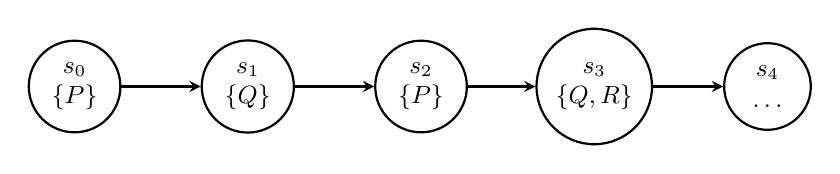
\begin{tikzpicture}[
      st/.style={draw, circle, minimum size=1.1cm, font=\small, align=center, thick},
      arr/.style={->, >=stealth, thick}
    ]
    \node[st] (s0) at (0, 0) {$s_0$\\$\{P\}$};
    \node[st] (s1) at (2.2, 0) {$s_1$\\$\{Q\}$};
    \node[st] (s2) at (4.4, 0) {$s_2$\\$\{P\}$};
    \node[st] (s3) at (6.6, 0) {$s_3$\\$\{Q, R\}$};
    \node[st] (s4) at (8.8, 0) {$s_4$\\$\dots$};

    \draw[arr] (s0) to (s1);
    \draw[arr] (s1) to (s2);
    \draw[arr] (s2) to (s3);
    \draw[arr] (s3) to (s4);
  \end{tikzpicture}
  \captionof{figure}{Trace $\sigma$ satisfying $(P \lor Q) U R$ with the existential witness at step 3.}
  \label{fig:until-trace-ex}
\end{center}

\begin{itemize}
    \item For $j = 3$, $R \in s_3$, satisfying the existential part of Until.
    \item For $k \in \{0, 1, 2\}$, we have $P \in s_0$ (so $P \lor Q$ holds), $Q \in s_1$ ($P \lor Q$ holds), and $P \in s_2$ ($P \lor Q$ holds).
    \item Thus, $\sigma \models (P \lor Q) U R$ is \textbf{True}.
\end{itemize}
If we modify the trace to $\sigma' = \{P\} \emptyset \{R\} \{P, R\}^\omega$, evaluating at $j=2$ requires checking $k=1$. Since $s_1' = \emptyset$, $P \lor Q$ is false. Thus, $\sigma' \not\models (P \lor Q) U R$ due to a universal violation at step 1.
\end{example}

\begin{example}[Reactivity / Response]
Let $\phi = G(r \implies F g)$, specifying that every request $r$ is eventually followed by a grant $g$ (where $AP = \{r, g\}$). Consider the trace $\sigma = \{r\} \{r\} \{r\} \{g\} \emptyset^\omega$, shown in Figure~\ref{fig:response-trace-ex}.

\begin{center}
  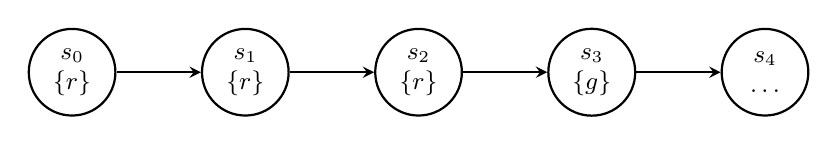
\begin{tikzpicture}[
      st/.style={draw, circle, minimum size=1.1cm, font=\small, align=center, thick},
      arr/.style={->, >=stealth, thick}
    ]
    \node[st] (s0) at (0, 0) {$s_0$\\$\{r\}$};
    \node[st] (s1) at (2.2, 0) {$s_1$\\$\{r\}$};
    \node[st] (s2) at (4.4, 0) {$s_2$\\$\{r\}$};
    \node[st] (s3) at (6.6, 0) {$s_3$\\$\{g\}$};
    \node[st] (s4) at (8.8, 0) {$s_4$\\$\dots$};

    \draw[arr] (s0) to (s1);
    \draw[arr] (s1) to (s2);
    \draw[arr] (s2) to (s3);
    \draw[arr] (s3) to (s4);
  \end{tikzpicture}
  \captionof{figure}{Trace $\sigma$ satisfying $G(r \implies F g)$.}
  \label{fig:response-trace-ex}
\end{center}

For $i \in \{0,1,2\}$, $r \in s_i$ and a grant occurs at $s_3$, so $F g$ holds. For $i \ge 3$, $r \notin s_i$, making the implication vacuously true. Hence, the trace satisfies $\phi$.
\end{example}

\begin{example}[Next-Step Formula]
Let $\phi = P \land (X Q \lor X X \neg R)$ over $AP = \{P, Q, R\}$. This formula states that at the initial position 0, $P$ must be true, and in the next step $Q$ must hold, or two steps later $R$ must be false.
We evaluate this formula over four distinct traces:
\begin{enumerate}
    \item \textbf{Trace $\sigma_A = \{P\}^\omega$} (illustrated in Figure~\ref{fig:next-trace-ex}):
          \begin{center}
            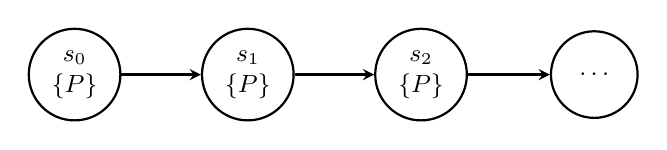
\begin{tikzpicture}[
                st/.style={draw, circle, minimum size=1.1cm, font=\small, align=center, thick},
                arr/.style={->, >=stealth, thick}
              ]
              \node[st] (s0) at (0, 0) {$s_0$\\$\{P\}$};
              \node[st] (s1) at (2.2, 0) {$s_1$\\$\{P\}$};
              \node[st] (s2) at (4.4, 0) {$s_2$\\$\{P\}$};
              \node[st] (s3) at (6.6, 0) {$\dots$};
              \draw[arr] (s0) to (s1);
              \draw[arr] (s1) to (s2);
              \draw[arr] (s2) to (s3);
            \end{tikzpicture}
            \captionof{figure}{Trace $\sigma_A$ satisfying the next-step formula.}
            \label{fig:next-trace-ex}
          \end{center}
          Evaluation at position 0:
          \begin{itemize}
              \item $P \in s_0 \implies$ True.
              \item $\sigma_A, 1 \models Q \implies$ False (since $Q \notin s_1$). Thus, $\sigma_A, 0 \models X Q$ is False.
              \item $\sigma_A, 2 \models \neg R \implies$ True (since $R \notin s_2$). Thus, $\sigma_A, 0 \models X X \neg R$ is True.
              \item The disjunction is True, so $\sigma_A \models \phi$ is \textbf{True}.
          \end{itemize}
    \item \textbf{Trace $\sigma_B = \{P, Q\}^\omega$}:
          Evaluation at position 0:
          \begin{itemize}
              \item $P \in s_0 \implies$ True.
              \item $\sigma_B, 1 \models Q \implies$ True. Thus, $\sigma_B, 0 \models X Q$ is True.
              \item The disjunction is True, so $\sigma_B \models \phi$ is \textbf{True}.
          \end{itemize}
    \item \textbf{Trace $\sigma_C = \{P, R\}^\omega$}:
          Evaluation at position 0:
          \begin{itemize}
              \item $P \in s_0 \implies$ True.
              \item $\sigma_C, 1 \models Q \implies$ False, so $\sigma_C, 0 \models X Q$ is False.
              \item $\sigma_C, 2 \models \neg R \implies$ False (since $R \in s_2$), so $\sigma_C, 0 \models X X \neg R$ is False.
              \item The disjunction is False, so $\sigma_C \not\models \phi$ (\textbf{False}).
          \end{itemize}
    \item \textbf{Trace $\sigma_D = \{Q, R\}^\omega$}:
          Evaluation at position 0:
          \begin{itemize}
              \item $P \in s_0 \implies$ False (since $P \notin s_0$).
              \item Thus, $\sigma_D \not\models \phi$ (\textbf{False}).
          \end{itemize}
\end{enumerate}
\end{example}

\begin{example}[Nested Eventually]
Let $\phi = F(P \land F Q)$ over $AP = \{P, Q\}$. This formula states that there is some state in the future (including the present) where $P$ holds, and from that state forward (including the same state), $Q$ eventually holds. Essentially, $P$ must be followed by $Q$.
We evaluate this over four traces:
\begin{enumerate}
    \item \textbf{Trace $\sigma_1 = \{Q\}\{Q\}\{Q\}\{P\}\{P\}^\omega$}:
          At index 3, $P$ holds. However, for any $j \ge 3$, $Q$ is never true. Thus, $F Q$ is false at index 3, and the formula is \textbf{False}.
    \item \textbf{Trace $\sigma_2 = \{P\}\{P\}\{P\}\{Q\}\{Q\}^\omega$}:
          At index 0, $P$ is true, and there is a future index (index 3) where $Q$ is true. Thus, the formula is \textbf{True}.
    \item \textbf{Trace $\sigma_3 = \emptyset \emptyset \{P, Q\} \emptyset^\omega$}:
          At index 2, both $P$ and $Q$ hold. Since the present is part of the future under the semantics of Eventually, $F Q$ is true at index 2, making $P \land F Q$ true at index 2. Since index 2 is reachable from index 0, the formula is \textbf{True}.
    \item \textbf{Trace $\sigma_4 = \{P\}^\omega$}:
          Since $Q$ never holds at any index, $F Q$ is always false. The formula is \textbf{False}.
\end{enumerate}
\end{example}

\begin{example}[Stabilization / Persistence]
Let $\phi = F G Q$ over $AP = \{P, Q\}$. This specifies that eventually $Q$ becomes true and remains true forever. This represents system stabilization.
\begin{enumerate}
    \item \textbf{Trace $\sigma_A = \{P\}\{Q\}\{P\}\{Q\}^\omega$}:
          At index 3, $G Q$ holds because $Q$ is true at all $j \ge 3$. Thus, $F G Q$ holds at index 0. The formula is \textbf{True}.
    \item \textbf{Trace $\sigma_B = \{P, Q\}^\omega$}:
          Since $Q$ is true globally, $G Q$ holds at index 0, so $F G Q$ is \textbf{True}.
    \item \textbf{Trace $\sigma_C = (\{Q\}\{Q\}\{P\})^\omega$}:
          No matter how far we go, there is always a future state containing $\{P\}$ (where $Q$ is false). Thus, $G Q$ never holds at any index, so $F G Q$ is \textbf{False}.
\end{enumerate}
\end{example}

\begin{example}[Liveness / Infinitely Many Times]
Let $\phi = G F P$. This formula requires $P$ to hold infinitely many times.
\begin{itemize}
    \item \textbf{Connection to S1S}: In Monadic Second-Order Logic, this infinite visitation is written as:
          \[
            \forall x \, \exists y \ge x : P(y)
          \]
          In LTL, the combination $G F$ mirrors this: the outer $G$ acts as the universal quantifier $\forall x$, and the inner $F$ acts as the existential quantifier $\exists y \ge x$.
    \item \textbf{Trace $\sigma_A = \{P\}\{Q\}\{P\}\{Q\}^\omega$}:
          $P$ only holds at indices 0 and 2. It does not hold infinitely many times. The formula is \textbf{False}.
    \item \textbf{Trace $\sigma_B = (\{Q\}\{Q\}\{P\})^\omega$}:
          $P$ holds at indices $2, 5, 8, \dots$ which are infinitely many times. The formula is \textbf{True}.
\end{itemize}
\end{example}

\subsection{Declarative vs. Operational Ordering Blow-Up}
A key benefit of LTL is its declarative nature: it specifies \emph{what} properties must hold without describing the operational tracking of states. This allows for extremely compact formulas where ordering is left implicit. However, compiling these formulas to operational representations (such as automata) forces the explicit representation of all possible state interleavings, leading to exponential size blow-ups.

Consider the formula:
\[
  \psi = \bigwedge_{i=1}^n F P_i
\]
which requires that each atomic proposition $P_i$ (for $i \in \{1, \dots, n\}$) must eventually hold.
\begin{itemize}
    \item \textbf{LTL representation}: The size of $\psi$ is linear in $n$ ($\mathcal{O}(n)$).
    \item \textbf{Automata representation}: A Büchi automaton recognizing the language of $\psi$ must explicitly keep track of which propositions have already been visited. It must branch to accommodate all $n!$ possible arrival orders of the events $P_i$. Thus, the state space of the automaton is of size $\mathcal{O}(2^n)$, representing the power set of $\{P_1, \dots, P_n\}$. This illustrates the declarative-to-operational gap.
\end{itemize}

% =======================================================================
\section{Expressive Power and Boundaries}
\label{sec:ltl-expressivity}

LTL is a powerful specification language, but it has strict expressive boundaries.

\subsection{Kamp's Theorem}
Kamp's landmark theorem (1968) establishes the expressive equivalence of linear-time formalisms:
\begin{theorem}[Kamp]
\label{thm:kamp}
Let $L \subseteq \Sigma^\omega$ be an $\omega$-language. The following are equivalent:
\begin{enumerate}
    \item $L$ is definable by an LTL formula.
    \item $L$ is definable by a first-order formula over the signature $(\mathbb{N}, 0, +1, <, \{Q_a\}_{a\in\Sigma})$.
    \item $L$ is a star-free $\omega$-regular language.
\end{enumerate}
\end{theorem}

\subsection{The Modulo Counting Barrier}
A key consequence of Kamp's Theorem is that LTL cannot perform modulo counting. 

\begin{proposition}[Non-LTL-Definable Language]
The language $L = \{ \sigma \in (2^{\{P\}})^{\omega} \mid \forall i \ge 0, (i \text{ is even}) \implies P \in s_i \}$ is not definable in LTL.
\end{proposition}
\begin{proof}[Intuition]
To recognize $L$, an automaton must count modulo 2 (alternating between even and odd positions) while accepting any valuation on odd steps. This unconstrained modulo cycle prevents the language from being counter-free, placing it outside the star-free regular languages.
\end{proof}

Conversely, if the states at odd positions are also constrained, we can express the alternation locally:
\begin{proposition}[LTL-Definable Alternation]
The language $L' = \{ \sigma \in (2^{\{P\}})^{\omega} \mid \forall i \ge 0, P \in s_i \iff i \text{ is even} \}$ is definable in LTL by the formula:
\[
  \phi_{L'} = P \land G (P \iff X \neg P)
\]
\end{proposition}

% =======================================================================
\section{Linear Temporal Logic with Past}
\label{sec:ltl-past}

To make specifications more compact, LTL can be extended with past-time operators, yielding $\text{LTL}+\text{P}$.

\subsection{Syntax and Semantics}
The past-time operators are Yesterday ($Y_s$, strong previous), Weak Yesterday ($Y_w$), and Since ($S$, past-time counterpart of Until):
\begin{align*}
  \sigma, i &\models Y_s \phi &&\iff i > 0 \text{ and } \sigma, i-1 \models \phi \\
  \sigma, i &\models Y_w \phi &&\iff i = 0 \text{ or } (i > 0 \text{ and } \sigma, i-1 \models \phi) \\
  \sigma, i &\models \phi_1 S \phi_2 &&\iff \exists j \in [0, i] \text{ s.t. } \sigma, j \models \phi_2 \text{ and } \forall k \in [j+1, i], \sigma, k \models \phi_1
\end{align*}
We derive Once ($O \phi \equiv \top S \phi$) and Historically ($H \phi \equiv \neg O \neg \phi$).

\paragraph{Unrolling Rules for Past Operators.}
Just like future temporal operators, past operators satisfy expansion recurrence relations looking backward in time:
\begin{align*}
  \phi_1 S \phi_2 &\equiv \phi_2 \lor (\phi_1 \land Y_s(\phi_1 S \phi_2)) \\
  O \phi &\equiv \phi \lor Y_s(O \phi) \\
  H \phi &\equiv \phi \land Y_w(H \phi)
\end{align*}

\paragraph{The Initial-State Anchor.}
The weak yesterday operator applied to false acts as a unique filter identifying the start of time:
\[
  \sigma, i \models Y_w \bot \iff i = 0
\]
This allows formulas evaluating in the past to detect when they have reached the initial state, serving as a boundary anchor during backward unrolling.

\paragraph{Extended Closure for $\text{LTL}+\text{P}$.}
To support the translation of formulas with past operators to automata, we define the \emph{extended closure} $Cl_{ex}(\psi)$ of an $\text{LTL}+\text{P}$ formula $\psi$ as the smallest set containing $\psi$ such that:
\begin{enumerate}
    \item If $\chi \in Cl_{ex}(\psi)$, then $\neg\chi \in Cl_{ex}(\psi)$ (with $\neg\neg\alpha \equiv \alpha$).
    \item If $\chi_1 \land \chi_2$ or $\chi_1 \lor \chi_2 \in Cl_{ex}(\psi)$, then $\chi_1, \chi_2 \in Cl_{ex}(\psi)$.
    \item If $X \chi \in Cl_{ex}(\psi)$, then $\chi \in Cl_{ex}(\psi)$.
    \item If $Y_s \chi$ or $Y_w \chi \in Cl_{ex}(\psi)$, then $\chi \in Cl_{ex}(\psi)$.
    \item If $\chi_1 U \chi_2 \in Cl_{ex}(\psi)$, then $\chi_1, \chi_2 \in Cl_{ex}(\psi)$ and $X(\chi_1 U \chi_2) \in Cl_{ex}(\psi)$.
    \item If $\chi_1 R \chi_2 \in Cl_{ex}(\psi)$, then $\chi_1, \chi_2 \in Cl_{ex}(\psi)$ and $X(\chi_1 R \chi_2) \in Cl_{ex}(\psi)$.
    \item If $\chi_1 S \chi_2 \in Cl_{ex}(\psi)$, then $\chi_1, \chi_2 \in Cl_{ex}(\psi)$ and $Y_s(\chi_1 S \chi_2) \in Cl_{ex}(\psi)$.
\end{enumerate}

\subsection{Gabbay's Equivalence vs. Succinctness}
Past operators do not add expressive power, but they make formulas exponentially smaller.
\begin{theorem}[Gabbay's Separation Theorem]
$\text{LTL}+\text{P}$ is expressively equivalent to pure-future LTL.
\end{theorem}

\begin{theorem}[Succinctness of $\text{LTL}+\text{P}$]
\label{thm:succinctness}
$\text{LTL}+\text{P}$ is exponentially more succinct than pure-future LTL.
\end{theorem}

\begin{proof}
For each $n \ge 1$, let $AP_n = \{P_0, \dots, P_n\}$. We define the language family $A_n \subseteq (2^{AP_n})^\omega$:
\[
  A_n = \left\{ w \in (2^{AP_n})^\omega \;\middle|\; \forall i \ge 0 : \left( \left[ \bigwedge_{j=1}^n \left( P_j \in w_i \iff P_j \in w_0 \right) \right] \implies \left( P_0 \in w_i \iff P_0 \in w_0 \right) \right) \right\}
\]
That is, any state $i$ that agrees with the initial state on $\{P_1, \dots, P_n\}$ must also agree on $P_0$.

\medskip\noindent
\textbf{1. Linear $\text{LTL}+\text{P}$ Formula.} We can define $A_n$ in $\text{LTL}+\text{P}$ with a formula of size $\mathcal{O}(n)$:
\[
  \phi_n = G \left( \bigwedge_{j=1}^n \left( P_j \iff O( Y_w \bot \land P_j ) \right) \implies \left( P_0 \iff O( Y_w \bot \land P_0 ) \right) \right)
\]
Since $Y_w \bot$ anchors the evaluation to index $0$, $O(Y_w \bot \land P_j)$ retrieves the value of $P_j$ at state 0.

\medskip\noindent
\textbf{2. Exponential Lower Bound for LTL.} We generalize $A_n$ to $B_n$, where any two matching states $i, j$ must agree on $P_0$:
\[
  B_n = \left\{ w \in (2^{AP_n})^\omega \;\middle|\; \forall i, j \ge 0 : \left( \left[ \bigwedge_{k=1}^n \left( P_k \in w_i \iff P_k \in w_j \right) \right] \implies \left( P_0 \in w_i \iff P_0 \in w_j \right) \right) \right\}
\]
\begin{lemma}[Connection Lemma]
If $A_n$ is definable by a pure-future LTL formula $\phi_n$ of size $f(n)$, then $B_n$ is definable by $\psi_n = G \phi_n$ of size $f(n) + 1$.
\end{lemma}
\begin{proof}
$w \models G \phi_n \iff \forall k \ge 0, w^{(k)} \models \phi_n$. Since $\phi_n$ defines $A_n$, this requires every suffix $w^{(k)}$ to satisfy the $A_n$ condition. This translates to verifying the implication for all pairs $k, k+i$, which is exactly the definition of $B_n$.
\end{proof}

\begin{lemma}
Any NBA recognizing $B_n$ must have at least $2^{2^n}$ states.
\end{lemma}
\begin{proof}
Let $L = 2^n$. Let $\bar{A} = S_0 S_1 \dots S_{L-1}$ be a finite word enumerating all possible subsets of $\{P_1, \dots, P_n\}$. 
For each subset $K \subseteq \{0, \dots, L-1\}$, define the word $\bar{A}_K$ by adding $P_0$ to states at indices in $K$. 
The infinite word $w_K = (\bar{A}_K)^\omega$ belongs to $B_n$ by construction.

Assume an NBA $\mathcal{B}$ recognizing $B_n$ has fewer than $2^{2^n}$ states. Then, by pigeonhole principle, there must be two distinct subsets $K \neq K'$ such that the runs of $\mathcal{B}$ on $w_K$ and $w_{K'}$ reach the same state $q_K = q_{K'}$ after reading the first block $\bar{A}_K$ and $\bar{A}_{K'}$.
This allows the automaton to accept the hybrid word $w^* = \bar{A}_{K'} \cdot (\bar{A}_K)^\omega$ (since the state runs merge at $q_K$).
However, because $K \neq K'$, there is some index $r$ where $r \in K'$ and $r \notin K$. Comparing positions $r$ and $L+r$ in $w^*$: they share the same $\{P_1, \dots, P_n\}$ signature $S_r$, but differ on $P_0$ ($P_0$ is true in the first block, false in the second). Thus, $w^* \notin B_n$, contradicting that $\mathcal{B}$ recognizes $B_n$. Hence, $\mathcal{B}$ must have at least $2^{2^n}$ states.
\end{proof}

The run merging logic is represented visually in Figure~\ref{fig:run-merging-ex}.

\begin{center}
  \begin{tikzpicture}[
      st/.style={draw, circle, minimum size=1.2cm, thick, font=\small},
      arr/.style={->, >=stealth, thick}
    ]
    % Separate runs diagram
    \begin{scope}
      \node[st, initial, initial where=left] (q0) at (0,0) {$q_0$};
      \node[st] (qk) at (2.2, 0.8) {$q_K$};
      \node[st] (qkp) at (2.2, -0.8) {$q_{K'}$};

      \draw[arr] (q0) to[bend left=15] node[above] {$\bar{A}_K$} (qk);
      \draw[arr] (q0) to[bend right=15] node[below] {$\bar{A}_{K'}$} (qkp);
      \draw[arr] (qk) edge[loop right] node {$(\bar{A}_K)^\omega$} (qk);
      \draw[arr] (qkp) edge[loop right] node {$(\bar{A}_{K'})^\omega$} (qkp);
    \end{scope}

    % Merged runs diagram
    \begin{scope}[xshift=6.5cm]
      \node[st, initial, initial where=left] (q0) at (0,0) {$q_0$};
      \node[st] (qm) at (2.5, 0) {$q_K = q_{K'}$};

      \draw[arr] (q0) to[bend left=25] node[above] {$\bar{A}_K$} (qm);
      \draw[arr] (q0) to[bend right=25] node[below] {$\bar{A}_{K'}$} (qm);
      \draw[arr] (qm) edge[loop above] node {$(\bar{A}_K)^\omega$} (qm);
      \draw[arr] (qm) edge[loop below] node {$(\bar{A}_{K'})^\omega$} (qm);
    \end{scope}
  \end{tikzpicture}
  \captionof{figure}{Run merging argument: if the NBA has fewer than $2^{2^n}$ states, two distinct runs on $w_K$ and $w_{K'}$ must merge at some state, causing the automaton to incorrectly accept the hybrid trace $w^*$.}
  \label{fig:run-merging-ex}
\end{center}

Combining the pieces: if $A_n$ were definable by a sub-exponential pure-future LTL formula $\phi_n$ ($|\phi_n| < 2^{cn}$), then $B_n$ would be definable by $\psi_n = G \phi_n$ of size $< 2^{cn} + 1$. Translating $\psi_n$ to an NBA would yield an automaton of size $2^{\mathcal{O}(|\psi_n|)} < 2^{2^n}$ for large $n$. This contradicts the $2^{2^n}$ lower bound. Thus, any pure-future LTL formula defining $A_n$ must be at least exponential in $n$.
\end{proof}

% =======================================================================
\section{LTL Satisfiability: The Tableau Construction}
\label{sec:ltl-tableau}

The LTL satisfiability problem is decided via a graph-based representation called the \emph{tableau}.

\paragraph{Whiteboard intuition: What is a Tableau?}
Imagine we are handed an LTL formula $\phi$ and asked: "Does there exist an infinite trace that satisfies this?" To answer this, we will build a massive state-space graph called the tableau. Every node in this graph will be a "candidate state" (called an atom) that contains a consistent set of formulas it claims are true. Edges will represent valid single-step time transitions.
If we can find an infinite path through this graph starting from a state that claims $\phi$ is true, we have found our model! However, there is a trap: to handle "eventually" properties (Beta formulas), nodes are allowed to postpone their obligations to the future. This means our graph will contain "spurious" paths that endlessly postpone promises and lie about the future. Our final job will be to filter out those lying paths.

\subsection{Negation Normal Form (NNF)}
In NNF, negations are pushed inward to literals. To negate Until formulas, we introduce the \emph{Release} operator ($R$), the dual of Until:
\[
  \phi_1 R \phi_2 \equiv \neg(\neg\phi_1 U \neg\phi_2)
\]
Semantically, $\phi_1 R \phi_2$ requires $\phi_2$ to hold up to and including the point where $\phi_1$ becomes true; if $\phi_1$ never holds, $\phi_2$ must hold forever.
The unrolling rule for Release is:
\[
  \phi_1 R \phi_2 \equiv \phi_2 \land (\phi_1 \lor X(\phi_1 R \phi_2))
\]

\subsection{Classification of Formulas: Alpha and Beta Formulas}
To systematically analyze formulas and build the tableau, we classify temporal and logical formulas in NNF into two categories based on their branching behavior: \textbf{Alpha} (universal/conjunctive) and \textbf{Beta} (existential/disjunctive) formulas.

\subsubsection{Alpha Formulas ($\alpha$)}
An alpha formula behaves like a conjunction: if it is true, all of its constituents must be true in the same state.
For each alpha formula $\alpha \in Cl(\phi)$, we define its constituent set $K(\alpha)$:
\begin{center}
\renewcommand{\arraystretch}{1.2}
\begin{tabular}{l|l}
Formula $\alpha$ & Constituent Set $K(\alpha)$ \\
\hline
$\psi_1 \land \psi_2$ & $\{\psi_1, \psi_2\}$ \\
$G \psi$ & $\{\psi, X G \psi\}$ \\
\end{tabular}
\end{center}
The semantic rule is that a state sequence $\sigma$ satisfies $\alpha$ at position $j$ if and only if it satisfies all formulas in $K(\alpha)$:
\[
  \sigma, j \models \alpha \iff \forall \chi \in K(\alpha), \; \sigma, j \models \chi
\]

\medskip\noindent
\textbf{Operational meaning of Alpha.} Alpha formulas are deterministic enforcements. There is no choice here. If you claim $\alpha$ is true today, you are strictly forced to also claim everything in $K(\alpha)$ is true today.

\subsubsection{Beta Formulas ($\beta$)}
A beta formula behaves like a disjunction: it introduces branching (non-determinism). If a beta formula holds, at least one of its two constituent sets must hold.
For each beta formula $\beta \in Cl(\phi)$, we define two constituent sets $K_1(\beta)$ and $K_2(\beta)$:
\begin{center}
\renewcommand{\arraystretch}{1.2}
\begin{tabular}{l|l|l}
Formula $\beta$ & First Set $K_1(\beta)$ & Second Set $K_2(\beta)$ \\
\hline
$\psi_1 \lor \psi_2$ & $\{\psi_1\}$ & $\{\psi_2\}$ \\
$F \psi$ & $\{\psi\}$ & $\{X F \psi\}$ \\
$\psi_1 U \psi_2$ & $\{\psi_2\}$ & $\{\psi_1, X(\psi_1 U \psi_2)\}$ \\
$\psi_1 R \psi_2$ & $\{\psi_1, \psi_2\}$ & $\{\psi_2, X(\psi_1 R \psi_2)\}$ \\
\end{tabular}
\end{center}
The semantic rule is that a state sequence $\sigma$ satisfies $\beta$ at position $j$ if and only if it satisfies all formulas in $K_1(\beta)$ or all formulas in $K_2(\beta)$:
\[
  \sigma, j \models \beta \iff \left( \forall \chi \in K_1(\beta), \; \sigma, j \models \chi \right) \lor \left( \forall \chi \in K_2(\beta), \; \sigma, j \models \chi \right)
\]

\medskip\noindent
\textbf{Operational meaning of Beta.} Beta formulas represent non-deterministic choices. For example, if you claim $F \psi$ is true today, you must choose a path: either fulfill it today by claiming $\psi$ is true now (First Set), or postpone the obligation by claiming $X F \psi$ is true, kicking the can to tomorrow (Second Set).

\subsection{Closure and Atoms}
\begin{definition}[Closure]
The closure $Cl(\phi)$ of an LTL formula $\phi$ in NNF is the smallest set of formulas containing $\phi$ such that:
\begin{enumerate}
    \item If $\chi \in Cl(\phi)$, then $\neg\chi \in Cl(\phi)$ (with $\neg\neg\alpha \equiv \alpha$).
    \item If $\chi_1 \land \chi_2$ or $\chi_1 \lor \chi_2 \in Cl(\phi)$, then $\chi_1, \chi_2 \in Cl(\phi)$.
    \item If $X \chi \in Cl(\phi)$, then $\chi \in Cl(\phi)$.
    \item If $\chi_1 U \chi_2 \in Cl(\phi)$, then $\chi_1, \chi_2 \in Cl(\phi)$ and $X(\chi_1 U \chi_2) \in Cl(\phi)$.
    \item If $\chi_1 R \chi_2 \in Cl(\phi)$, then $\chi_1, \chi_2 \in Cl(\phi)$ and $X(\chi_1 R \chi_2) \in Cl(\phi)$.
\end{enumerate}
\end{definition}
The size of $Cl(\phi)$ satisfies $|Cl(\phi)| \le 4|\phi|$.
\begin{definition}[$\phi$-Atom]
A $\phi$-atom is a subset $A \subseteq Cl(\phi)$ that satisfies the following three conditions:
\begin{enumerate}
    \item \textbf{Propositional completeness and consistency}: For every formula $\psi \in Cl(\phi)$, exactly one of $\{\psi, \neg \psi\}$ is in $A$. Moreover, $\top \in A$ and $\bot \notin A$.
    \item \textbf{Alpha consistency}: For every alpha formula $\alpha \in Cl(\phi)$, if $\alpha \in A$ then $K(\alpha) \subseteq A$. If $\alpha \notin A$, then $K(\alpha) \not\subseteq A$ (meaning at least one constituent is missing from $A$).
    \item \textbf{Beta consistency}: For every beta formula $\beta \in Cl(\phi)$, if $\beta \in A$ then $K_1(\beta) \subseteq A$ or $K_2(\beta) \subseteq A$. If $\beta \notin A$, then both $K_1(\beta) \not\subseteq A$ and $K_2(\beta) \not\subseteq A$.
\end{enumerate}
\end{definition}

\paragraph{Basic Formulas.}
A formula is called \emph{basic} if it is an atomic proposition $p \in AP$ or a next-step formula $X \psi$. An important algebraic property of the closure is that a $\phi$-atom is uniquely determined by the truth values of its basic formulas. All non-basic formulas are reconstructed bottom-up by propagating the alpha and beta consistency rules. This reduces the search space of possible atoms from $2^{|Cl(\phi)|}$ to the combinations of truth assignments to the basic formulas (at most $2^k$, where $k$ is the number of basic formulas in the closure).

\subsection{Tableau Graph}
\begin{definition}[Tableau]
The tableau $T(\phi)$ is a directed graph $(V, E)$ where:
\begin{itemize}
    \item $V$ is the set of all $\phi$-atoms.
    \item $E \subseteq V \times V$ is the transition relation, defined as:
          \[
            (A, B) \in E \iff \forall X\chi \in Cl(\phi) : X\chi \in A \iff \chi \in B
          \]
\end{itemize}
\end{definition}

\medskip\noindent
\textbf{Operational meaning of the Tableau.} Operationally, the tableau is a massive graph where every node is a candidate state of our system (an atom), and edges represent valid single-step transitions forward in time. An edge exists from $A$ to $B$ if and only if all the "tomorrow" promises made in $A$ ($X\chi$) are kept "today" in $B$ ($\chi$). Finding a model for our formula reduces to finding a valid infinite path through this graph starting from an atom containing $\phi$.

% =======================================================================
\section{Fulfilling Paths and SCS Reduction}
\label{sec:ltl-fulfilling}

An infinite path in $T(\phi)$ is a sequence of atoms $\pi = A_0 A_1 A_2 \dots$ with $(A_i, A_{i+1}) \in E$.

\subsection{Induced Paths and the Infinite Postponement Problem}
Does every path in the tableau correspond to a real LTL model? To answer this, we look at the concept of an \emph{induced path}.

If we are given an actual, true LTL model $\sigma = s_0 s_1 s_2 \dots$ that satisfies $\phi$, we can trace its exact footprint through the tableau. For each step $i$, we define an atom $A_i$ containing exactly the formulas that are true at step $i$: $A_i = \{ \psi \in Cl(\phi) \mid \sigma, i \models \psi \}$. Because $\sigma$ is a real model, this sequence of atoms $A_0 A_1 A_2 \dots$ is guaranteed to be a valid path in $T(\phi)$. We say the model $\sigma$ \emph{induces} this path. This proves a critical property: \textbf{the tableau does not lose anything.} Any valid model lives inside the tableau as an induced path.

But the reverse is not true! There is an asymmetry. Consider the trace where $P$ is always true: $\sigma = \{P\}^\omega$. Now, let's try to evaluate the formula $F \neg P$. In the tableau, an atom might claim $F \neg P$ is true by using the Beta non-determinism to choose $X F \neg P$ (postponing the obligation to tomorrow). At the next step, it postpones again. And again. The tableau allows this infinite chain of postponements because it only enforces local step-by-step consistency. Thus, the tableau contains a "spurious" path that endlessly kicks the can down the road, claiming $F \neg P$ is true but never actually delivering $\neg P$. This is the \emph{infinite postponement problem}.

Because of this asymmetry, we must filter the paths in the tableau. We only want paths that don't lie about the future.

\subsection{Fulfilling Paths}

\begin{definition}[Promising Formulas and Fulfilling Paths]
A formula $\psi \in Cl(\phi)$ is \emph{promising} if it is of the form $\alpha U \beta$. It promises $\beta$.
An atom $A$ \emph{fulfills} $\psi$ if $\neg \psi \in A$ or $\beta \in A$.
A path $\pi$ is \emph{fulfilling} if for every promising formula $\psi \in Cl(\phi)$, $\pi$ contains infinitely many atoms that fulfill $\psi$.
\end{definition}

\begin{theorem}[Fulfilling Path Theorem]
\label{thm:fulfilling-path}
An LTL formula $\phi$ is satisfiable if and only if there exists a fulfilling path $\pi = A_0 A_1 \dots$ in $T(\phi)$ such that $\phi \in A_0$.
\end{theorem}
\begin{proof}
($\implies$) Let $\sigma = s_0 s_1 \dots$ be an LTL model satisfying $\phi$. Define the path $\pi = A_0 A_1 \dots$ by setting $A_i = \{ \chi \in Cl(\phi) \mid \sigma, i \models \chi \}$. 
Propositional, local, and temporal consistency follow from LTL semantics, so each $A_i$ is an atom. Edge consistency holds because $X\chi \in A_i \iff \sigma, i \models X\chi \iff \sigma, i+1 \models \chi \iff \chi \in A_{i+1}$.
If $\alpha U \beta \in A_i$, then $\sigma, i \models \alpha U \beta$, meaning there is some $j \ge i$ where $\sigma, j \models \beta$, so $\beta \in A_j$, which fulfills the promise. Thus, $\pi$ is fulfilling.

\medskip\noindent
($\impliedby$) Let $\pi = A_0 A_1 \dots$ be a fulfilling path with $\phi \in A_0$. Define the model $\sigma = s_0 s_1 \dots$ by setting $s_i = A_i \cap AP$. We prove by induction on the structure of $\psi \in Cl(\phi)$ that $\sigma, i \models \psi \iff \psi \in A_i$.
The base case ($\psi = p \in AP$), negation, and conjunction steps follow immediately from the definition of $\sigma$ and propositional consistency of atoms.
\begin{itemize}
    \item \textbf{Next Step} ($\psi = X \chi$):
          $\sigma, i \models X \chi \iff \sigma, i+1 \models \chi \iff \chi \in A_{i+1}$ (by induction hypothesis) $\iff X\chi \in A_i$ (by edge relation $A_i \to A_{i+1}$).
    \item \textbf{Until Step} ($\psi = \alpha U \beta$):
          \begin{itemize}
              \item If $\alpha U \beta \in A_i$: since $\pi$ is fulfilling, there is a smallest index $j \ge i$ such that $A_j$ fulfills the promise. If $j=i$, we must have $\beta \in A_i$ (otherwise $\neg(\alpha U \beta) \in A_i$, a contradiction). By induction hypothesis, $\sigma, i \models \beta$, so $\sigma, i \models \alpha U \beta$.
                    If $j > i$, then for all $k \in [i, j-1]$, $A_k$ does not fulfill the promise, so $\beta \notin A_k$, forcing $\alpha \in A_k$ and $X(\alpha U \beta) \in A_k$ by the temporal consistency rule. By edge transition, this propagates to $\alpha U \beta \in A_j$. Since $A_j$ is fulfilling, $\beta \in A_j$, meaning $\sigma, j \models \beta$. By induction hypothesis, $\sigma, k \models \alpha$ for all $k \in [i, j-1]$. Thus, $\sigma, i \models \alpha U \beta$.
              \item If $\alpha U \beta \notin A_i$: then $\neg(\alpha U \beta) \in A_i$. By temporal consistency, $\neg \beta \in A_i$ and $\neg X(\alpha U \beta) \in A_i$. Inductively, this propagates: if $\beta$ were true at any future step $j \ge i$, we would have $\beta \in A_j$, contradicting the propagation of $\neg \beta$. Thus, $\sigma, i \not\models \alpha U \beta$. \qedhere
          \end{itemize}
\end{itemize}
\end{proof}

\subsection{Reduction to Reachable Strongly Connected Subgraphs}
Searching for infinite fulfilling paths on a finite graph reduces to strongly connected subgraphs (SCS).

\begin{definition}[Fulfilling SCS]
A strongly connected subgraph $S \subseteq T(\phi)$ is non-transient if it contains at least one cycle. A non-transient SCS $S$ is fulfilling if for every promising formula $\alpha U \beta \in Cl(\phi)$ and every node $u \in S$:
\[
  \alpha U \beta \in u \implies \exists v \in S \text{ such that } \beta \in v
\]
\end{definition}

\begin{theorem}
An LTL formula $\phi$ is satisfiable if and only if the tableau $T(\phi)$ contains a fulfilling SCS $S$ reachable from some initial atom $A_0$ containing $\phi$.
\end{theorem}

If such an SCS exists, we can construct an \emph{ultimately periodic model} of the form $u \cdot v^\omega$.

\subsection{Tableau Pruning Rules}
Instead of checking all SCSs, we partition the graph into Maximal Strongly Connected Subgraphs (MSCS) and apply two pruning rules:
\begin{enumerate}
    \item \textbf{Reachability Pruning}: Delete all states not reachable from a $\phi$-atom.
    \item \textbf{Terminal MSCS Pruning}: An MSCS $S$ is terminal if it has no outgoing transitions to states outside $S$. If a terminal MSCS is not fulfilling, prune it entirely. Since it is terminal, a path cannot leave it, and since it is not fulfilling, it cannot contain any valid infinite path.
\end{enumerate}

\subsection{Detailed Case Study: $\phi = \Box P \land \Diamond \neg P$}
We verify the unsatisfiability of $\phi = \Box P \land \Diamond \neg P$ (written in NNF).
The closure is $Cl(\phi) = \{ \phi, \neg\phi, \Box P, \neg\Box P, \Diamond\neg P, \neg\Diamond\neg P, P, \neg P, X\Box P, \neg X\Box P, X\Diamond\neg P, \neg X\Diamond\neg P \}$.
We identify the 8 atoms based on the basic formulas $P$, $X\Box P$, and $X\Diamond\neg P$:

\begin{center}
\renewcommand{\arraystretch}{1.2}
\begin{tabular}{c|ccc|ccc|l}
  Atom & $P$ & $X\Box P$ & $X\Diamond\neg P$ & $\Box P$ & $\Diamond\neg P$ & $\phi$ & Promises \\
  \hline
  $A_0$ & 0 & 0 & 0 & 0 & 1 & 0 & $\Diamond\neg P, \neg\Box P$ \\
  $A_1$ & 0 & 0 & 1 & 0 & 1 & 0 & $\Diamond\neg P, \neg\Box P$ \\
  $A_2$ & 0 & 1 & 0 & 0 & 1 & 0 & $\Diamond\neg P, \neg\Box P$ \\
  $A_3$ & 0 & 1 & 1 & 0 & 1 & 0 & $\Diamond\neg P, \neg\Box P$ \\
  $A_4$ & 1 & 0 & 0 & 0 & 0 & 0 & $\neg\Box P$ \\
  $A_5$ & 1 & 0 & 1 & 0 & 1 & 0 & $\Diamond\neg P, \neg\Box P$ \\
  $A_6$ & 1 & 1 & 0 & 1 & 0 & 0 & None \\
  $A_7$ & 1 & 1 & 1 & 1 & 1 & 1 & $\Diamond\neg P$ \\
\end{tabular}
\end{center}

Applying the transition relation:
\begin{itemize}[nosep]
  \item From $\{A_0, A_4\}$, where $X\Box P=0$ and
  $X\Diamond\neg P=0$, transitions go to $\{A_4\}$.
  \item From $\{A_1, A_5\}$, where $X\Box P=0$ and
  $X\Diamond\neg P=1$, transitions go to
  $\{A_0, A_1, A_2, A_3, A_5\}$.
  \item From $\{A_2, A_6\}$, where $X\Box P=1$ and
  $X\Diamond\neg P=0$, transitions go to $\{A_6\}$.
  \item From $\{A_3, A_7\}$, where $X\Box P=1$ and
  $X\Diamond\neg P=1$, transitions go to $\{A_7\}$.
\end{itemize}

\begin{figure}[ht]
  \centering
  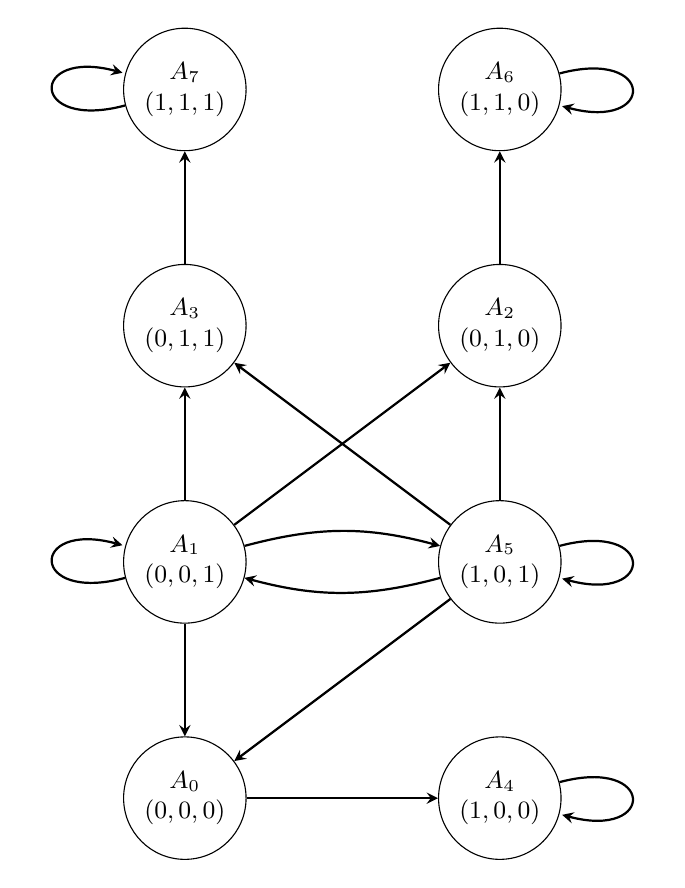
\begin{tikzpicture}[
      st/.style={draw, circle, minimum size=1.5cm, font=\small, align=center},
      arr/.style={->, >=stealth, thick}
    ]
    \node[st] (A7) at (0, 0)   {$A_7$\\$(1,1,1)$};
    \node[st] (A6) at (4, 0)   {$A_6$\\$(1,1,0)$};
    \node[st] (A3) at (0,-3)   {$A_3$\\$(0,1,1)$};
    \node[st] (A2) at (4,-3)   {$A_2$\\$(0,1,0)$};
    \node[st] (A1) at (0,-6)   {$A_1$\\$(0,0,1)$};
    \node[st] (A5) at (4,-6)   {$A_5$\\$(1,0,1)$};
    \node[st] (A0) at (0,-9)   {$A_0$\\$(0,0,0)$};
    \node[st] (A4) at (4,-9)   {$A_4$\\$(1,0,0)$};

    \draw[arr] (A7) edge[loop left] (A7);
    \draw[arr] (A6) edge[loop right] (A6);
    \draw[arr] (A4) edge[loop right] (A4);
    \draw[arr] (A3) to (A7);
    \draw[arr] (A2) to (A6);
    \draw[arr] (A0) to (A4);

    \draw[arr] (A1) edge[loop left] (A1);
    \draw[arr] (A1) to[bend left=15] (A5);
    \draw[arr] (A1) to (A3);
    \draw[arr] (A1) to (A2);
    \draw[arr] (A1) to (A0);

    \draw[arr] (A5) edge[loop right] (A5);
    \draw[arr] (A5) to[bend left=15] (A1);
    \draw[arr] (A5) to (A3);
    \draw[arr] (A5) to (A2);
    \draw[arr] (A5) to (A0);
  \end{tikzpicture}
  \caption{Tableau graph for $\phi = \Box P \land \Diamond \neg P$. The node labels represent the basic variables $(P, X\Box P, X\Diamond\neg P)$.}
  \label{fig:tableau-case-study}
\end{figure}

The only state containing $\phi$ is $A_7$. The only path starting from $A_7$ is $A_7^\omega$. However, $A_7^\omega$ contains the promising formula $\Diamond \neg P$, which is never fulfilled because $\neg P$ is false in $A_7$ (where $P=1$). Thus, no fulfilling path starting from a $\phi$-state exists: $\phi$ is unsatisfiable.

% =======================================================================
\section{Automata-Theoretic Translation}
\label{sec:ltl-automata}

We compile LTL with past formulas directly into Generalized B\"uchi Automata.

\begin{definition}[GNBA for $\text{LTL}+\text{P}$]
Given an $\text{LTL}+\text{P}$ formula $\psi$, we define the GNBA $\mathcal{A}_\psi = (Q, \Sigma, I, \Delta, \mathcal{F})$:
\begin{enumerate}
    \item $\Sigma = 2^{AP}$.
    \item $Q$ is the set of all propositionally, locally, and temporally consistent atoms over $Cl_{ex}(\psi)$.
    \item $I = \{ S \in Q \mid \psi \in S \text{ and } \forall Y\alpha \in Cl_{ex}(\psi), Y\alpha \notin S \}$.
    \item $(S, S') \in \Delta$ on symbol $a$ iff:
          \begin{itemize}
              \item $P \in a \iff P \in S$ (for all $p \in AP$).
              \item $X \alpha \in S \iff \alpha \in S'$.
              \item $Y \alpha \in S' \iff \alpha \in S$.
          \end{itemize}
    \item $\mathcal{F} = \{ F_{\alpha U \beta} \mid \alpha U \beta \in Cl_{ex}(\psi) \}$ where $F_{\alpha U \beta} = \{ S \in Q \mid \beta \in S \lor \neg(\alpha U \beta) \in S \}$.
\end{enumerate}
\end{definition}

To translate the GNBA with acceptance sets $\{F_1, \dots, F_k\}$ to a standard NBA, we apply a counter construction:
\begin{align*}
  Q' &= Q \times \{1, \dots, k\} \\
  I' &= I \times \{1\} \\
  F' &= Q \times \{k\}
\end{align*}
The transition relation advances the counter from $i$ to $(i \bmod k) + 1$ if and only if the current state belongs to $F_i$.

% =======================================================================
\paragraph{Bridge to Chapter~\ref{ch:ltl-mc-fairness}.}
This chapter stops at the specification side: syntax, semantics, expressiveness, past operators, satisfiability, and the automata viewpoint.  Chapter~\ref{ch:ltl-mc-fairness} takes the next step and uses those formulas for model checking over finite systems, with fairness handled there.

% =======================================================================
\section{Exercises}
\label{sec:ltl-exercises}

\begin{chapex}[Weak Yesterday Nesting]
Let $\sigma$ be a state sequence.
\begin{enumerate}
    \item Prove that $\sigma, i \models Y_w \bot \iff i = 0$.
    \item Show that $\sigma, i \models Y_w(Y_w(Y_w \bot)) \iff i \le 2$.
    \item Write an $\text{LTL}+\text{P}$ formula that holds at position $i$ if and only if $i > 2$.
\end{enumerate}
\end{chapex}
\begin{proof}[Solution]
\begin{enumerate}
    \item By the semantic definition of the weak yesterday operator:
          \[
            \sigma, i \models Y_w \bot \iff i = 0 \lor (i > 0 \text{ and } \sigma, i-1 \models \bot)
          \]
          Since $\sigma, i-1 \models \bot$ is false for any suffix position, the second disjunct is always false. Thus:
          \[
            \sigma, i \models Y_w \bot \iff i = 0
          \]
    \item Let $\psi_0 = \bot$ and $\psi_k = Y_w \psi_{k-1}$ for $k \ge 1$. We show by induction on $k$ that $\sigma, i \models \psi_k \iff i \le k - 1$.
          \begin{itemize}
              \item \textbf{Base Case} ($k=1$): $\sigma, i \models Y_w \bot \iff i \le 0 \iff i=0$, which is true by part 1.
              \item \textbf{Inductive Step}: Assume the property holds for $k$, i.e., $\sigma, i \models \psi_k \iff i \le k - 1$. For $k+1$:
                    \[
                      \sigma, i \models Y_w \psi_k \iff i = 0 \lor (i > 0 \text{ and } \sigma, i-1 \models \psi_k)
                    \]
                    By the induction hypothesis, $\sigma, i-1 \models \psi_k \iff i-1 \le k - 1 \iff i \le k$.
                    Therefore, the satisfaction condition becomes:
                    \[
                      i = 0 \lor (i > 0 \text{ and } i \le k) \iff i \le k
                    \]
                    which matches $i \le (k+1) - 1$. This completes the induction.
          \end{itemize}
          Setting $k=3$, we obtain $\sigma, i \models Y_w(Y_w(Y_w \bot)) \iff i \le 2$.
    \item The condition $i > 2$ is the exact negation of the condition $i \le 2$. Using the formula derived in part 2, the desired formula is:
          \[
            \phi = \neg Y_w(Y_w(Y_w \bot))
          \]
\end{enumerate}
\end{proof}

\begin{chapex}[Omega-Regular Conversion]
Consider the LTL formula $\phi = P U G Q$ over $AP = \{P, Q\}$. Write the equivalent $\omega$-regular expression over $\Sigma = 2^{AP}$.
\end{chapex}
\begin{proof}[Solution]
The alphabet is $\Sigma = \{\emptyset, \{P\}, \{Q\}, \{P,Q\}\}$. We partition $\Sigma$ as $\Sigma_P = \{\{P\}, \{P,Q\}\}$ and $\Sigma_Q = \{\{Q\}, \{P,Q\}\}$. 
The Until requires a suffix where $G Q$ holds, meaning all states belong to $\Sigma_Q$. Before this suffix, $P$ must hold, meaning all states belong to $\Sigma_P$. 
Thus, the equivalent expression is:
\[
  L(\phi) = (\Sigma_P)^* (\Sigma_Q)^\omega = (\{P\} + \{P,Q\})^* (\{Q\} + \{P,Q\})^\omega
\]
\end{proof}

\begin{chapex}[LTL Rewrite]
Rewrite $\phi = G (P U Q)$ using only boolean operators, $X$, $F$, and $G$, but without using $U$. Prove the equivalence.
\end{chapex}
\begin{proof}[Solution]
The equivalent formula is $\phi' = G(P \lor Q) \land G F Q$.
\begin{itemize}
    \item ($\implies$) Let $\sigma \models G(P U Q)$. Let $i \ge 0$. Since $\sigma, i \models P U Q$, there is $j \ge i$ where $Q \in s_j$, so $F Q$ holds. Since $i$ is arbitrary, $G F Q$ holds. By the unrolling rule, $\sigma, i \models Q \lor (P \land X(P U Q))$, which implies $P \lor Q$ holds. Thus, $G(P \lor Q)$ holds.
    \item ($\impliedby$) Let $\sigma \models G(P \lor Q) \land G F Q$. Let $i \ge 0$. Since $G F Q$ holds, let $j \ge i$ be the first step where $Q$ holds. For all $k \in [i, j-1]$, $Q$ is false. Since $P \lor Q$ holds globally, we must have $P$ true at all $k \in [i, j-1]$. Thus, $\sigma, i \models P U Q$. Since $i$ is arbitrary, $G(P U Q)$ holds.
\end{itemize}
\end{proof}
